\section{Calibration of laser photon flux}

The calibration of the absolute laser photon flux was performed with the use of the silicon photodiode Hamamatsu S2281.
The tabulated quantum efficiency of this diode at the wavelength of our laser ($\lambda=470$ nm) is 62.6\%. 
The active part of the diode is a circle with a diameter of 11.3~mm, which is 100~mm$^2$. 
A KEITHLEY 6485 picoammeter was used to measure the average diode current while illuminated by the laser beam.
The noise diode current was estimated to be at the level of 0.2~pA. 
During the MAPMT characterization, the laser frequency was maintained at 20 kHz. 
For light calibration, the higher the frequency, the better the current measurement accuracy that can be achieved from the point of view of the noise level. 
The maximum frequency of our laser is 1 MHz.
However, there are additional systematic uncertainties associated with the extrapolation from one frequency to another. 
For this reason, the scan of the light field was done at a working frequency of 20 kHz. 
The measured current in the center position of the laser head was around 29.2~pA at this frequency, meaning the systematic uncertainty
of this measurement was below 1\%.  We made a detailed two-dimensional scan of the photon flux by
moving the laser head with step sizes of 2~mm in the X and Y directions along the full area where the 3 MAPMTs were located during the characterization procedure.
Normalized to one laser pulse and 1~mm$^2$ area, the number of photons with $\lambda=470$~nm  is presented in Fig.~\ref{fig:light_flux}.
The maximum value of the photon flux in the center of the light field equals 145 $\gamma/mm^2/pulse$.
These measurements were done without  any optical filters installed. We used neutral density calibrated optical filters with anti-reflection coating.
To check the possible filter effects, we made a measurement of the light flux for one of the filters with a tabulated attenuation of 100. 
This test was done with a frequency of 1 MHz to increase the accuracy of the current measurement. 
The ratio of the measured attenuation factor to that tabulated was determined to be 1.05$\pm 0.01$. This coefficient was applied to the map of the photon flux when used for data with optical filters. It takes into account the possible effects of rescattering or reflection of the photons by the filters.
\begin{figure}[h]
\centering
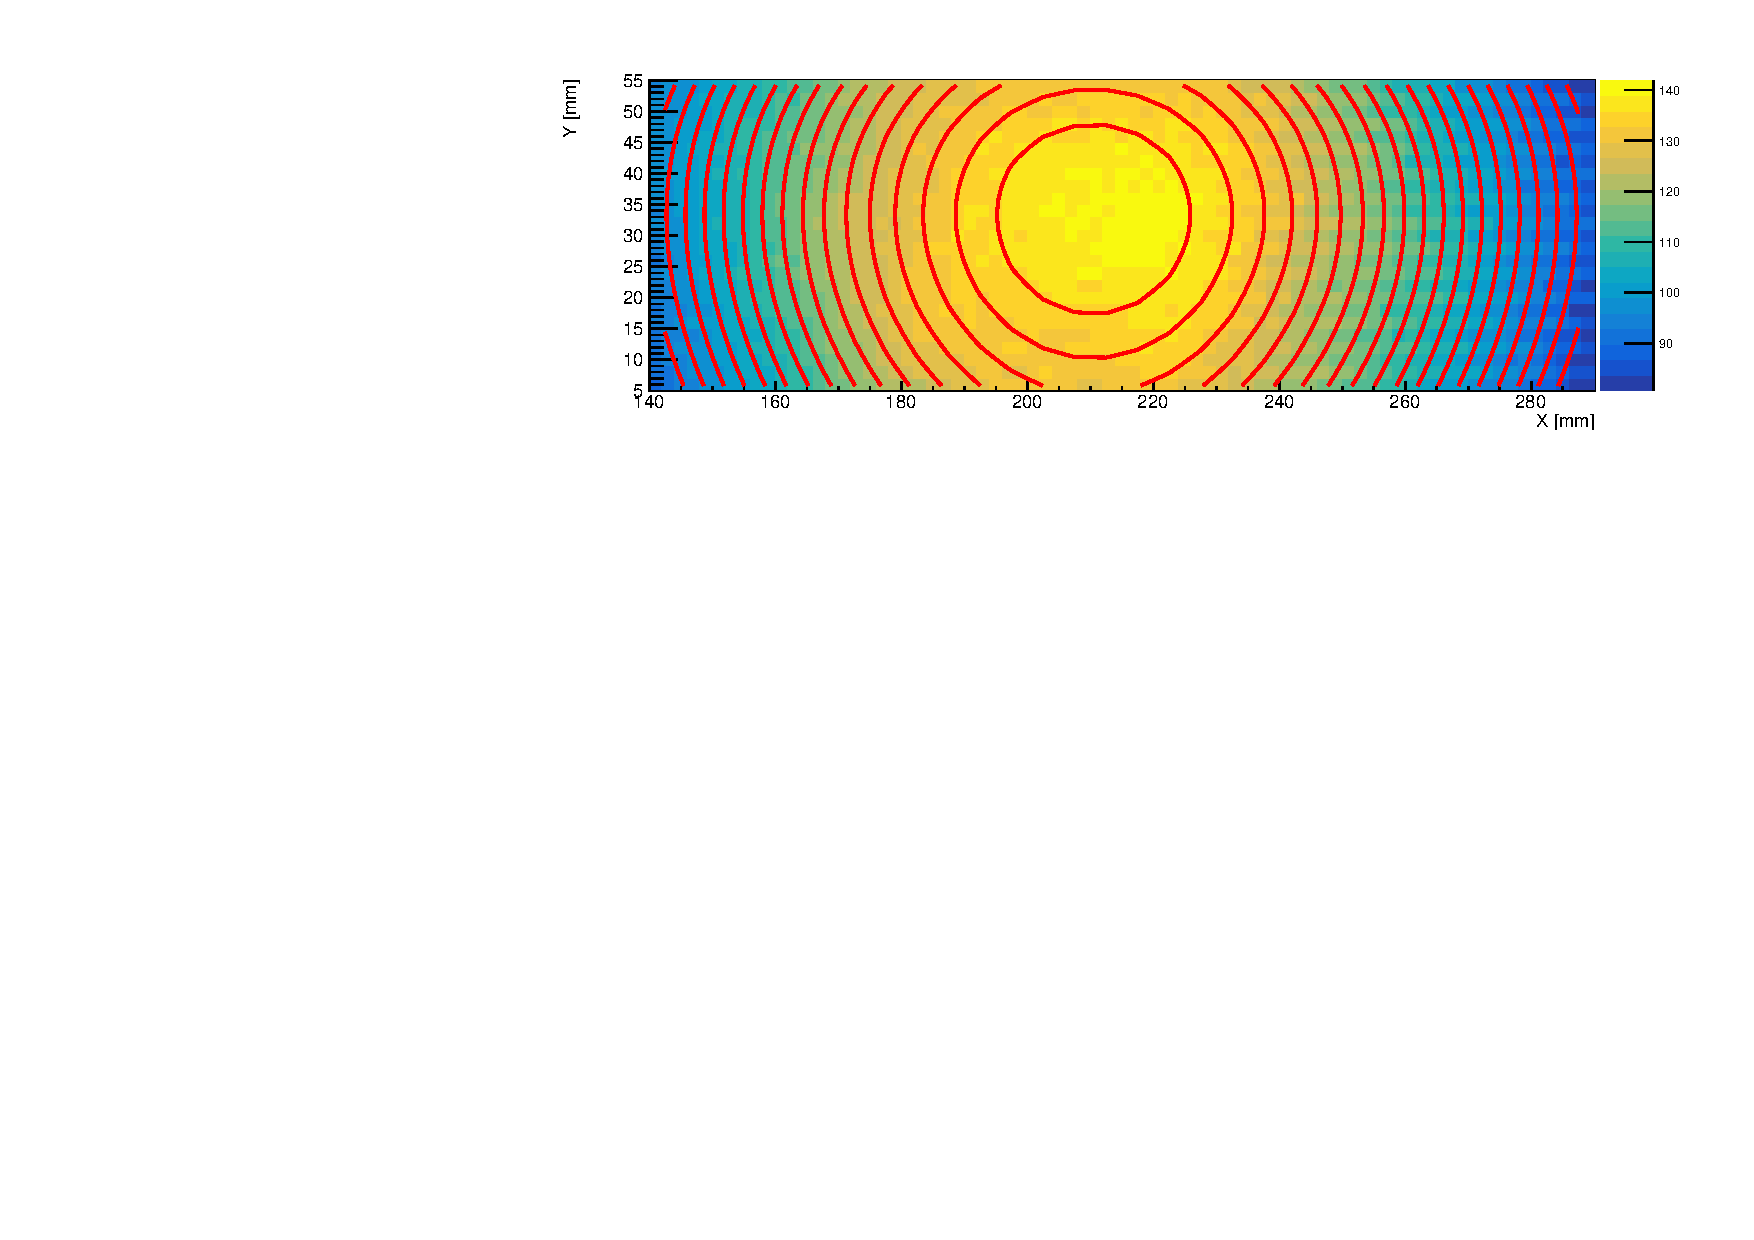
\includegraphics[width=0.5\textwidth]{figures/photon_flux.pdf}
\caption{Number of photons per mm$^2$ in  one laser pulse.}
\label{fig:light_flux}
\end{figure}

The knowledge of the absolute number of photons hitting the photomultiplier tubes during the characterization gave us the possibility to measure the quantum efficiency of the MAPMTs for each pixel. The average number of photoelectrons, $\mu$, is proportional to the quantum efficiency:
$$
\mu=\epsilon_{QE} \int_{S_{pixel}}\frac {dN_\gamma}{dS} dS,
$$
\noindent
where $\int_{S_{pixel}}\frac {dN_\gamma}{dS} dS$ is the number of photons integrated over the pixel's area, $S_{pixel}$, and $\epsilon_{QE}$ is the quantum efficiency of the pixel.
The integration included the measured light field at the position of the pixel under study.
The parameter $\mu$ was determined during the PMT characterization.